\documentclass[ 12pt ]{article}
\usepackage{amsmath, amsthm, amssymb, csquotes, enumitem, graphicx, listings, mathrsfs, xcolor}
\usepackage[margin=0.5in]{geometry}
\graphicspath{ ./ }

\begin{document}

\noindent Landon Fox \\
\noindent CS 487 \\
\noindent March 14, 2021

\begin{center}
	\Large Homework 2
\end{center}

\begin{enumerate}
	% problem 1
	\item[\textbf{1.}] Let $\textbf{f} : \mathbb{R}^3 \to \mathbb{R}^2$ be defined as $$\textbf{f}(\textbf{x}) = \begin{bmatrix} \sum_{i=0}^2 x_i \sin x_{(i+2)\mathrm{mod}\;3} \\[6pt]
		\sum_{i=0}^2 \sin x_i \cos x_{(i+1)\mathrm{mod}\;3}\end{bmatrix}.$$ Calculate the Jacobian of $\textbf{f}$.

		\begin{proof}[Solution]
			Let $\textbf{f} : \mathbb{R}^3 \to \mathbb{R}^2$ be defined as
			\begin{align*}
				\textbf{f}(\textbf{x}) &= \begin{bmatrix} \sum_{i=0}^2 x_i \sin x_{(i+2)\mathrm{mod}\;3} \\[6pt] \sum_{i=0}^2 \sin x_i \cos x_{(i+1)\mathrm{mod}\;3} \end{bmatrix} \\
				&= \sum_{i=0}^2 \begin{bmatrix} x_i \sin x_{(i+2)\mathrm{mod}\;3} \\ \sin x_i \cos x_{(i+1)\mathrm{mod}\;3} \end{bmatrix} \\
				\textbf{f}(\textbf{x}) &= \begin{bmatrix} x_0 \sin x_2 + x_1 \sin x_0 + x_2 \sin x_1 \\ \sin x_0 \cos x_1 + \sin x_1 \cos x_2 + \sin x_2 \cos x_0 \end{bmatrix}.
			\end{align*}
			Further, let $D\textbf{f}$ denote the Jacobian. Observe that
			\begin{align*}
				D\textbf{f}(\textbf{x}) &= \begin{bmatrix} \frac{\partial \textbf{f}_1}{\partial x_0} & \frac{\partial \textbf{f}_1}{\partial x_1} & \frac{\partial \textbf{f}_1}{\partial
					x_2} \\[6pt] \frac{\partial \textbf{f}_2}{\partial x_0} & \frac{\partial \textbf{f}_2}{\partial x_1} & \frac{\partial \textbf{f}_2}{\partial x_2} \end{bmatrix} \\
				&= \begin{bmatrix} \sin x_2 + x_1 \cos x_0 & \sin x_0 + x_2 \cos x_1 & \sin x_1 + x_0 \cos x_2 \\ \cos x_0 \cos x_1 - \sin x_2 \sin x_0 & \cos x_1 \cos x_2 - \sin x_0
					\sin x_1 & \cos x_2 \cos x_0 - \sin x_1 \sin x_2 \end{bmatrix}.
			\end{align*}
		\end{proof}


	% problem 2
	\item[\textbf{2.}] Suppose we have an input feature defined as $\textbf{x} = \begin{bmatrix} 2 & -5 & 1 \end{bmatrix}^t \in \mathbb{R}^3$ and a trained two layer linear classifier
		with the following weights and biases. $$W_1 = \begin{bmatrix} 1 & 2 & 3 \\ -4 & -2 & 1 \\ 1 & -2 & -3 \end{bmatrix},\; \textbf{b}_1 = \begin{bmatrix} -2 \\ -1 \\ 3
		\end{bmatrix}\;\;\; \mathrm{and}\;\;\; W_2 = \begin{bmatrix} -2 & -3 & -1 \\ 3 & 1 & 2 \end{bmatrix},\; \textbf{b}_2 = \begin{bmatrix} 3 \\ 1 \end{bmatrix}.$$
		\begin{enumerate}
			\item[\textbf{a.}] Write the full equation of this classifier.
			\item[\textbf{b.}] Calculate the output of this classifier.
			\item[\textbf{c.}] Which class does this classifier label the input $\textbf{x}$ as? Why?
			\item[\textbf{d.}] Assuming the first class was the correct class for the the feature vector $\textbf{x}$, calculate the hinge loss for the classifier.
			\item[\textbf{e.}] Assuming the first class was the correct class for the the feature vector $\textbf{x}$, calculate the softmax loss for the classifier.
		\end{enumerate}

		\begin{proof}[Solution]
			Suppose $\textbf{x}, \textbf{b}_1 \in \mathbb{R}^3$, $\textbf{b}_2 \in \mathbb{R}^2$, $W_1 \in \mathbb{R}^{3 \times 3}$, $W_2 \in \mathbb{R}^{2 \times 3}$ are all defined as
			stated above.
			\begin{enumerate}
				\item[\textbf{a.}] Let $\textbf{f} : \mathbb{R}^3 \to \mathbb{R}^3,\; \textbf{g} : \mathbb{R}^3 \to \mathbb{R}^2$ be defined as $$\textbf{f}(\textbf{x}) = W_1 \textbf{x}
					+ \textbf{b}_1\;\;\; \mathrm{and}\;\;\; \textbf{g}(\textbf{x}) = W_2 \textbf{x} + \textbf{b}_2.$$ Observe that the expression of our classifier is $(\textbf{gf})(
					\textbf{x})$. Hence,
					\begin{align*}
						(\textbf{gf})(\textbf{x}) &= \textbf{g}(W_1 \textbf{x} + \textbf{b}_1) \\
						&= W_2 W_1 \textbf{x} + W_2 \textbf{b}_1 + \textbf{b}_2 \\
						&= \begin{bmatrix} -2 & -3 & -1 \\ 3 & 1 & 2 \end{bmatrix} \begin{bmatrix} 1 & 2 & 3 \\ -4 & -2 & 1 \\ 1 & -2 & -3 \end{bmatrix} \textbf{x} +
							\begin{bmatrix} -2 & -3 & -1 \\ 3 & 1 & 2 \end{bmatrix} \begin{bmatrix} -2 \\ -1 \\ 3 \end{bmatrix} + \begin{bmatrix} 3 \\ 1 \end{bmatrix} \\
						(\textbf{gf})(\textbf{x}) &= \begin{bmatrix} 9 & 4 & -6 \\ 1 & 0 & 4 \end{bmatrix} \textbf{x} + \begin{bmatrix} 7 \\ 0 \end{bmatrix}.
					\end{align*}

				\item[\textbf{b.}] Now that we have the expression of the classifier, the output provided $\textbf{x}$ is $$(\textbf{gf})(\textbf{x}) = \begin{bmatrix} 9 & 4 & -6 \\ 1 &
					0 & 4 \end{bmatrix} \begin{bmatrix} 2 \\ -5 \\ 1 \end{bmatrix} + \begin{bmatrix} 7 \\ 0 \end{bmatrix} = \begin{bmatrix} -1 \\ 6 \end{bmatrix}.$$

				\item[\textbf{c.}] After observing the resulting output, $\begin{bmatrix} -1 & 6 \end{bmatrix}^t$, we can see that the score is -1 and 6 for class one and two,
					respectively. Therefore, according to the classifier, $\textbf{x}$ is more akin to class two since score of class two exceeds that of class one and so $\textbf{x}$
					would be classified as class two.

				\item[\textbf{d.}] Assuming that class one was the correct class for $\textbf{x}$, the hinge loss can be calculated as $$L_1 = \sum_{j \neq 1} \max \{ 0, s_j - s_1 +
					1 \} = \max \{ 0, s_2 - s_1 + 1 \} = \max \{ 0, 6 - (-1) + 1 \} = 8.$$

				\item[\textbf{e.}] Again, assuming that class one was the correct class for $\textbf{x}$, the softmax loss can be calculated as $$L_1 = -\ln \frac{e^{s_1}}{\sum_{j
					} e^{s_j}} = -\ln \frac{e^{-1}}{e^{-1} + e^6} = \ln (1 + e^7) \approx 7.$$
			\end{enumerate}
		\end{proof}


	% problem 3
	\item[\textbf{3.}] Using the classifier from \textbf{2}, use an activation layer with the function $\sigma(x) = \frac{1}{1 + e^{-x}}$ after the linear combination and bias additions.
		\begin{enumerate}
			\item[\textbf{a.}] Draw the computational graph of the network.
			\item[\textbf{b.}] Perform the forward pass on the graph with the input vector $\textbf{x} = \begin{bmatrix} 2 & 3 & 4 \end{bmatrix}^t$.
			\item[\textbf{c.}] Calculate $\nabla_W L$ though the backward pass of the backpropagation procedure.
		\end{enumerate}

		\begin{proof}[Solution]
			Let $\pmb{\sigma}(\textbf{x}) = \frac{1}{1 + e^{-\textbf{x}}}$ denote the component-wise sigmoid function.
			\begin{enumerate}
				\item[\textbf{a.}] Refer to the computational graph in \textbf{3b}.

				\item[\textbf{b.}] Consider the following definitions,
					\begin{align*}
						\pmb{\eta} &= W_1 \textbf{x}, \\
						\pmb{\lambda} &= \pmb{\eta} + \textbf{b}_1, \\
						\pmb{\mu} &= \pmb{\sigma}(\pmb{\lambda}), \\
						\pmb{\psi} &= W_2 \pmb{\mu}, \\
						\pmb{\omega} &= \pmb{\psi} + \textbf{b}_2, \\
						\textbf{L} &= \pmb{\sigma}(\pmb{\omega}).
					\end{align*}
					Defining $\textbf{x} = \begin{bmatrix} 2 & 3 & 4 \end{bmatrix}^t$ and performing a forward pass on the graph, we obtain the following.
					\begin{center}
						\includegraphics{capture}
					\end{center}

				\item[\textbf{c.}] We will be assuming that the backpropagation will be applied to the result of the classifier. Provided the definitions stated above, we can see that
					the local gradients evaluate to
					\begin{align*}
						\frac{\partial \textbf{L}_i}{\partial \pmb{\omega}_j} &= \begin{cases} (1 - \sigma(\pmb{\omega}_i))\sigma(\pmb{\omega}_i); & i = j \\ 0; & i \neq j, \end{cases} \\
						\frac{\partial \pmb{\omega}_i}{\partial \pmb{\psi}_j} &= \begin{cases} 1; & i = j \\ 0; & i \neq j, \end{cases} \\
						\frac{\partial \pmb{\psi}_i}{\partial W_{2jk}} &= \begin{cases} \pmb{\mu}_k; & i = j \\ 0; & i \neq j, \end{cases} \\
						\frac{\partial \pmb{\psi}_i}{\partial \pmb{\mu}_j} &= W_{2ij}, \\
						\frac{\partial \pmb{\mu}_i}{\partial \pmb{\lambda}_j} &= \begin{cases} (1 - \sigma(\pmb{\lambda}_i))\sigma(\pmb{\lambda}_i); & i = j \\ 0; & i \neq j, \end{cases} \\
						\frac{\partial \pmb{\lambda}_i}{\partial \pmb{\eta}_j} &= \begin{cases} 1; & i = j \\ 0; & i \neq j ,\end{cases} \\
						\frac{\partial \pmb{\eta}_i}{\partial W_{1jk}} &= \begin{cases} \textbf{x}_k; & i = j \\ 0; & i \neq j. \end{cases}
					\end{align*}
					Now we calculate $\nabla_{W_1} \textbf{L}$ and $\nabla_{W_2} \textbf{L}$. Moreover,
					\begin{align*}
						(\nabla_{W_{1jk}} \textbf{L})_i &= \frac{\partial \textbf{L}_i}{\partial \pmb{\omega}_i} \frac{\partial \pmb{\omega}_i}{\partial \pmb{\psi}_i} \frac{
						\partial \pmb{\psi}_i}{\partial \pmb{\mu}_j} \frac{\partial \pmb{\mu}_j}{\partial \pmb{\lambda}_j} \frac{\partial \pmb{\lambda}_j}{\partial
						\pmb{\eta}_j} \frac{\partial \pmb{\eta}_j}{\partial W_{1jk}} \\
						&= (1 - \sigma(\pmb{\omega}_i))\sigma(\pmb{\omega}_i) W_{2ij}(1 - \sigma(\pmb{\lambda}_j)) \sigma(\pmb{\lambda}_j) \textbf{x}_k \\
						(\nabla_{W_{1jk}} \textbf{L})_i &= (1 - \textbf{L}_i)\textbf{L}_i(1 - \pmb{\mu}_j)\pmb{\mu}_j W_{2ij}\textbf{x}_k
					\end{align*} accounting for the cases when partial derivatives are zero. Similarly, $$(\nabla_{W_{2jk}} \textbf{L})_i = \frac{\partial
					\textbf{L}_i}{\partial \pmb{\omega}_i} \frac{\partial \pmb{\omega}_i}{\partial \pmb{\psi}_i} \frac{\partial \pmb{\psi}_i}{\partial  W_{2jk}} =
					(1 - \sigma(\pmb{\omega}_i))\sigma(\pmb{\omega}_i)\pmb{\mu}_k = (1 - \textbf{L}_i)\textbf{L}_i \pmb{\mu}_k.$$
					Then after utilizing each component of $\textbf{L}$ and weight $w_{ijk}$, we obtain the following
					$$(\nabla_{W_1} \textbf{L})_1 \approx \begin{bmatrix} 0 & 0 & 0 \\ -2 \times 10^{-5} & 5 \times 10^{-5} & -1 \times 10^{-5} \\ -9 \times 10^{-7} & 2 \times 10^{-6} &
					-4 \times 10^{-7} \end{bmatrix},\;\; (\nabla_{W_1} \textbf{L})_2 \approx \begin{bmatrix} 0 & 0 & 0 \\ 7 \times 10^{-7} & -2 \times 10^{-6} & 3 \times 10^{-7} \\ 2 \times
					10^{-7} & -4 \times 10^{-7} & 9 \times 10^{-8} \end{bmatrix},$$
					$$(\nabla_{W_1} \textbf{L})_1 \approx \begin{bmatrix} 0.2 & 3 \times 10^{-6} & 4 \times 10^{-7} \\ 0.2 & 3 \times 10^{-6} & 4 \times 10^{-7} \end{bmatrix},\;\;
					(\nabla_{W_1} \textbf{L})_2 \approx \begin{bmatrix} 0.02 & 3 \times 10^{-7} & 4 \times 10^{-8} \\ 0.02 & 3 \times 10^{-7} & 4 \times 10^{-8} \end{bmatrix}.$$
			\end{enumerate}
		\end{proof}


	% problem 4
	\item[\textbf{4.}] \textbf{The XOR Problem.} The linear classification with one layer fails to solve the problem of classifying objects that represent a population whose probabilities
		resemble the XOR function. That is, in a two dimensional feature space, one population occupies the first and third quadrants, while the other population occupies the second and
		fourth quadrants. \\
		In this problem, we will implement a two layer neural network to address the problem of classifying classes who represent the XOR property. In order to accomplish this task we
		will write a program to perform the following.
		\begin{enumerate}
			\item[] \textbf{Data Generation}: We will create a data set of samples in two dimensions belonging to the x-class and the o-class.
			\item[] \textbf{Data Visualization}: We will plot the data in a scatter plot.
			\item[] \textbf{Network Setup}: We will set up a network with two layers. We will use Keras for the purpose of establishing, training, and evaluating our model.
			\item[] \textbf{Model Training}: We will train the network using a predefined loss function, an optimization algorithm, etc.
			\item[] \textbf{Model Accuracy}: We will generate another dataset of samples and labels for testing purposes. We will then evaluate the trained model on this test dataset and
				present and discuss the results.
		\end{enumerate}

		\begin{proof}[Solution] $ $
			\begin{enumerate}
				\item[\textbf{a.}] $ $
					\begin{lstlisting}[basicstyle=\ttfamily\footnotesize, numbers=left, tabsize=4, frame=single, breaklines=true, postbreak=\mbox{\textcolor{red}{$\hookrightarrow$}\space}]
import numpy as np
import matplotlib.pyplot as plt

def get_2d_samples( n, x_low, x_high, y_low, y_high ):
  return np.append(
    np.expand_dims( ( x_high - x_low ) * np.random.rand( n ) + x_low, axis=1 ),
    np.expand_dims( ( y_high - y_low ) * np.random.rand( n ) + y_low, axis=1 ),
    axis=1
  )

n = 250

low = -1
high = 20

x_label = [ 1, 0 ]
x_class = np.append(
  get_2d_samples( n, -high, -low, low, high ),
  get_2d_samples( n, low, high, -high, -low ),
  axis=0
)
x_labels = np.full( ( 2 * n, 2 ), x_label )

o_label = [ 0, 1 ]
o_class = np.append(
  get_2d_samples( n, low, high, low, high ),
  get_2d_samples( n, -high, -low, -high, -low ),
  axis=0
)
o_labels = np.full( ( 2 * n, 2 ), o_label )

plt.scatter( x_class[ :, 0 ], x_class[ :, 1 ], marker='+', c='blue', label='X-class' )
plt.scatter( o_class[ :, 0 ], o_class[ :, 1 ], marker='o', c='red', edgecolors='none', label='O-class' )
plt.legend()
plt.grid( True )
					\end{lstlisting}
					\begin{center}
						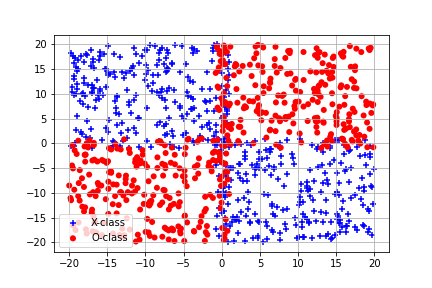
\includegraphics{index}
					\end{center}

				\item[\textbf{b.}] $ $
					\begin{lstlisting}[basicstyle=\ttfamily\footnotesize, numbers=left, tabsize=4, frame=single, breaklines=true, postbreak=\mbox{\textcolor{red}{$\hookrightarrow$}\space}]
def unison_shuffle( arr1, arr2 ):
  assert len( arr1 ) == len( arr2 )
  p = np.random.permutation( len( arr1 ) )
  return arr1[ p ], arr2[ p ]

train_data = np.append( x_class, o_class, axis=0 )
train_labels = np.append( x_labels, o_labels, axis=0 )
train_data, train_labels = unison_shuffle( train_data, train_labels )
					\end{lstlisting}

				\item[\textbf{c.}] $ $
					\begin{lstlisting}[basicstyle=\ttfamily\footnotesize, numbers=left, tabsize=4, frame=single, breaklines=true, postbreak=\mbox{\textcolor{red}{$\hookrightarrow$}\space}]
import tensorflow as tf
from keras.models import Sequential
from keras.layers import Dense

model = Sequential( name="sequential" )
model.add( Dense( 8, activation='relu',    name='hidden', input_shape=(2,) ) )
model.add( Dense( 2, activation='sigmoid', name='output' ) )

m = model( tf.ones( ( 0, 2 ) ) )

model.summary()
print( model.get_weights() )
					\end{lstlisting}
					\begin{lstlisting}[basicstyle=\ttfamily\footnotesize, numbers=left, tabsize=4, frame=single, breaklines=true, postbreak=\mbox{\textcolor{red}{$\hookrightarrow$}\space}]
Model: "sequential"
_________________________________________________________________
Layer (type)                 Output Shape              Param #   
=================================================================
hidden (Dense)               (None, 8)                 24        
_________________________________________________________________
output (Dense)               (None, 2)                 18        
=================================================================
Total params: 42
Trainable params: 42
Non-trainable params: 0
_________________________________________________________________
[array([[-0.64198864, -0.31149253,  0.12465358,  0.51851094,  0.10364014,
        -0.2944944 , -0.6057409 ,  0.271675  ],
       [-0.15246111,  0.18977368, -0.74891365, -0.46075818,  0.06056041,
         0.56482756, -0.28045   ,  0.4248793 ]], dtype=float32), array([0., 0., 0., 0., 0., 0., 0., 0.], dtype=float32), array([[-0.42965856,  0.28658497],
       [ 0.1367293 ,  0.66468215],
       [ 0.00855005, -0.70028514],
       [ 0.3539567 ,  0.34797347],
       [ 0.25254083,  0.2704208 ],
       [ 0.37440073, -0.6057212 ],
       [-0.1871522 ,  0.02674162],
       [ 0.54186773, -0.5938508 ]], dtype=float32), array([0., 0.], dtype=float32)]
					\end{lstlisting}

				\item[\textbf{d.}] $ $
					\begin{lstlisting}[basicstyle=\ttfamily\footnotesize, numbers=left, tabsize=4, frame=single, breaklines=true, postbreak=\mbox{\textcolor{red}{$\hookrightarrow$}\space}]
model.compile(
  optimizer='adam',
  loss='binary_crossentropy',
  metrics=[ 'accuracy' ]
)

model.fit( train_data, train_labels, batch_size=32, epochs=20, verbose=1 )
					\end{lstlisting}
					\begin{lstlisting}[basicstyle=\ttfamily\footnotesize, numbers=left, tabsize=4, frame=single, breaklines=true, postbreak=\mbox{\textcolor{red}{$\hookrightarrow$}\space}]
Epoch 1/20
32/32 [==============================] - 1s 1ms/step - loss: 0.8814 - accuracy: 0.5973
Epoch 2/20
32/32 [==============================] - 0s 1ms/step - loss: 0.7409 - accuracy: 0.6462
Epoch 3/20
32/32 [==============================] - 0s 1ms/step - loss: 0.6364 - accuracy: 0.7750
Epoch 4/20
32/32 [==============================] - 0s 1ms/step - loss: 0.5529 - accuracy: 0.8148
Epoch 5/20
32/32 [==============================] - 0s 1ms/step - loss: 0.4677 - accuracy: 0.8611
Epoch 6/20
32/32 [==============================] - 0s 1ms/step - loss: 0.4199 - accuracy: 0.8753
Epoch 7/20
32/32 [==============================] - 0s 1ms/step - loss: 0.3853 - accuracy: 0.8824
Epoch 8/20
32/32 [==============================] - 0s 1ms/step - loss: 0.3622 - accuracy: 0.8800
Epoch 9/20
32/32 [==============================] - 0s 1ms/step - loss: 0.3399 - accuracy: 0.8774
Epoch 10/20
32/32 [==============================] - 0s 1ms/step - loss: 0.3263 - accuracy: 0.8735
Epoch 11/20
32/32 [==============================] - 0s 1ms/step - loss: 0.3180 - accuracy: 0.8831
Epoch 12/20
32/32 [==============================] - 0s 1ms/step - loss: 0.3136 - accuracy: 0.8747
Epoch 13/20
32/32 [==============================] - 0s 1ms/step - loss: 0.2815 - accuracy: 0.8811
Epoch 14/20
32/32 [==============================] - 0s 1ms/step - loss: 0.2778 - accuracy: 0.8943
Epoch 15/20
32/32 [==============================] - 0s 1ms/step - loss: 0.2646 - accuracy: 0.8876
Epoch 16/20
32/32 [==============================] - 0s 1ms/step - loss: 0.2517 - accuracy: 0.8857
Epoch 17/20
32/32 [==============================] - 0s 1ms/step - loss: 0.2627 - accuracy: 0.8969
Epoch 18/20
32/32 [==============================] - 0s 1ms/step - loss: 0.2614 - accuracy: 0.8760
Epoch 19/20
32/32 [==============================] - 0s 1ms/step - loss: 0.2549 - accuracy: 0.8804
Epoch 20/20
32/32 [==============================] - 0s 1ms/step - loss: 0.2418 - accuracy: 0.9030
					\end{lstlisting}

				\item[\textbf{e.}] $ $
					\begin{lstlisting}[basicstyle=\ttfamily\footnotesize, numbers=left, tabsize=4, frame=single, breaklines=true, postbreak=\mbox{\textcolor{red}{$\hookrightarrow$}\space}]
k = 75

x_test_class = np.append(
  get_2d_samples( k, -high, -low, low, high ),
  get_2d_samples( k, low, high, -high, -low ),
  axis=0
)
x_test_labels = np.full( ( 2 * k, 2 ), x_label )

o_test_class = np.append(
  get_2d_samples( k, low, high, low, high ),
  get_2d_samples( k, -high, -low, -high, -low ),
  axis=0
)
o_test_labels = np.full( ( 2 * k, 2 ), o_label )

test_data = np.append( x_test_class, o_test_class, axis=0 )
test_labels = np.append( x_test_labels, o_test_labels, axis=0 )
test_data, test_labels = unison_shuffle( test_data, test_labels )

score = model.evaluate( test_data, test_labels, batch_size=32, verbose=1 )
print( score )
					\end{lstlisting}
					\begin{lstlisting}[basicstyle=\ttfamily\footnotesize, numbers=left, tabsize=4, frame=single, breaklines=true, postbreak=\mbox{\textcolor{red}{$\hookrightarrow$}\space}]
10/10 [==============================] - 0s 2ms/step - loss: 0.2654 - accuracy: 0.9233
[0.26535511016845703, 0.9233333468437195]
					\end{lstlisting}

				\item[\textbf{f.}] After training our neural network with our randomly generated XOR dataset, we can see that it works relatively well with accuracy $\sim 0.905$ and
					loss $\sim 0.195$; however, by no means does it meet industry standards. I believe this is because the features we are utilizing have an overlap on the interval
					$[-1, 1]$ for both the $x$ and $y$ axis. Moreover, this overlap makes it difficult to determine the class an input belongs to when it is likely that the decision
					boundaries lie on the $x$ and $y$ axis. The regions that constitute to a misclassification has an area of 156, when accounting for the area of the entire region,
					we obtain an approximate probability of 9.8\% of an arbitrary point being a member of the region. Observe that our loss is nearly double the aforementioned
					probability. \\
					In regard to sensitivity analysis, we will examine the effect taken on our network's accuracy when altering the number of samples from each class, dataset overlap,
					and batch size.
					\begin{center}
					
					\begin{tabular}{|c|c|c|}
						\hline
						Number of samples & Approximate loss & Approximate accuracy \\
						\hline
						100 & 0.68 & 0.73 \\
						250 & 0.20 & 0.91 \\
						1000 & 0.16 & 0.92 \\
						10000 & 0.14 & 0.93 \\
						\hline
					\end{tabular}
					\end{center}
					As illustrated in the table, increasing the sample size does appear to increase the accuracy quite slowly. More analysis would be required to determine precisely
					where the accuracy would converge. The benefit may not be worth the computational cost as exponential increase of samples has very little increase in performance.
					\begin{center}
					\begin{tabular}{|c|c|c|}
						\hline
						Units of overlap & Approximate loss & Approximate accuracy \\
						\hline
						-1 & 0.09 & 0.99 \\
						0 & 0.25 & 0.95 \\
						1 & 0.20 & 0.91 \\
						5 & 0.53 & 0.70 \\
						10 & 0.67 & 0.59 \\
						\hline
					\end{tabular}
					\end{center}
					As we might expect, when we remove the overlap between the classes, the model increases in its performance. Moreover, it comes as no surprise as the loss increases
					when the overlap increases.
					\begin{center}
					\begin{tabular}{|c|c|c|}
						\hline
						Batch size & Approximate loss & Approximate accuracy \\
						\hline
						1 & 0.15 & 0.92 \\
						10 & 0.18 & 0.91 \\
						25 & 0.23 & 0.92 \\
						50 & 0.40 & 0.89 \\
						100 & 0.51 & 0.85 \\
						\hline
					\end{tabular}
					\end{center}
					When altering the batch size we can see an overall trend of the loss increasing and the accuracy slowly decreasing. I would appear that for our specific model, the
					optimal batch size would lie between 1 and 25. More analysis would need to be conducted to find the exact optimum.
			\end{enumerate}
		\end{proof}
\end{enumerate}

\end{document}
